\subsection{Level2.1: $y=x^2$ について}
\subsubsection{プログラムソース(変更部分)}
steepest\_decent.cの一部を以下のように変更した
\begin{lstlisting}[basicstyle=\ttfamily\footnotesize, frame=single]
    /** 以下の式を編集して完成させよ(1) **/
    z = x*x;

    /** 以下の式を編集して完成させよ(2-1) **/
    z_dx = 2*x;
\end{lstlisting}
更に今のalphaの値が見やすいように以下の出力を追加した。
\begin{lstlisting}[basicstyle=\ttfamily\footnotesize, frame=single] 
     printf("alpha = %.2f\n",alpha);
\end{lstlisting}
\subsubsection{観察意図と観察方法}
刻み値をより小さくすると探索点がより細かく移動するため最適性は良くなるだろう。しかし,小さくしすぎると最適性は良いが探索回数が増えてしまい,効率性は悪くなるだろう。

上記のように予想してこれを検証するために,seed値を1に固定しalphaの値を変えることにより探索を行い,結果を観測する。
\subsubsection{実行結果}
alphaの値を0.1から0.1刻みに1まで実行した。以下に実行結果の一部を示す。
\begin{lstlisting}[basicstyle=\ttfamily\footnotesize, frame=single]
alpha = 0.10
~~~~
step 62 x -0.0000072277 y 5.1121064439 f(x,y) 0.0000000001 5.224013e-11
step 63 x -0.0000057822 y 5.1121064439 f(x,y) 0.0000000000 3.343369e-11
~~~~
step 74 x -0.0000004967 y 5.1121064439 f(x,y) 0.0000000000 2.466971e-13
FINISH 3 step 75 x and y were not updated.

alpha = 0.20
~~~~
step 27 x -0.0000075424 y 5.1121064439 f(x,y) 0.0000000001 5.688705e-11
step 28 x -0.0000045254 y 5.1121064439 f(x,y) 0.0000000000 2.047934e-11
~~~~
step 34 x -0.0000002111 y 5.1121064439 f(x,y) 0.0000000000 4.457906e-14
FINISH 3 step 35 x and y were not updated.

alpha = 0.40
~~~~
step 8 x -0.0000188653 y 5.1121064439 f(x,y) 0.0000000004 3.558982e-10
step 9 x -0.0000037731 y 5.1121064439 f(x,y) 0.0000000000 1.423593e-11
~~~~
step 12 x -0.0000000302 y 5.1121064439 f(x,y) 0.0000000000 9.110995e-16
FINISH 3 step 13 x and y were not updated.

alpha = 0.50
step 0 x -7.3692442371 y 5.1121064439 f(x,y) 54.3057606266 5.430576e+01
step 1 x 0.0000000000 y 5.1121064439 f(x,y) 0.0000000000 0.000000e+00
FINISH 3 step 2 x and y were not updated.

alpha = 0.60
~~~~
step 8 x -0.0000188653 y 5.1121064439 f(x,y) 0.0000000004 3.558982e-10
step 9 x 0.0000037731 y 5.1121064439 f(x,y) 0.0000000000 1.423593e-11
~~~~
step 12 x -0.0000000302 y 5.1121064439 f(x,y) 0.0000000000 9.110995e-16
FINISH 3 step 13 x and y were not updated.

alpha = 0.90
~~~~
step 62 x -0.0000072277 y 5.1121064439 f(x,y) 0.0000000001 5.224013e-11
step 63 x 0.0000057822 y 5.1121064439 f(x,y) 0.0000000000 3.343369e-11
~~~~
step 84 x -0.0000000533 y 5.1121064439 f(x,y) 0.0000000000 2.844223e-15
FINISH 3 step 85 x and y were not updated.

alpha = 1.00
FINISH 1 step 1000 this trial couldn't be search enough under the term_cond=1000.
\end{lstlisting}

alphaの値が0.1のときから徐々にstep数が減少していき,alpha=0.5で最もstep数が少なくなった。更にalphaの値を増やしていくとstep数が増加していった。
\subsubsection{考察}
各alpha値でf(x)の値が0になる箇所を示したが,f(x)の表示されている範囲の値が0になってから実行が終わるまでにかかったstep数がalpha=0.5から離れるに連れて多くなっていることがわかった。偏微分の値がほぼ0になるとxの値が0に近づいているということになるが,そこから実行されている回数が多いほど更に細かく見ているため最適性が良くなると思った。しかし最も最適性がよかったalpha値から少なくなるごとに最適性が悪くなっていき,alpha値が低くても最適性が良いというわけではなかった。しかし効率性に関しては予想通り悪くなっていた(下図\ref{fig:alpha0.2},\ref{fig:alpha0.4},\ref{fig:alpha0.5})。

逆にalpha値が大きくなっていくと探索回数が増えていき,alpha=1.0からは実行が1000回を超えてしまった(下図\ref{fig:alpha1.0})。

探索点の推移のグラフから,alpha=0.2の際はほぼ0になってそこから動くことが少なくなった時点で動作を終了しているが,alpha=0.5の際は運が良く一度の試行で最小値を導いていることがわかる(下図\ref{fig:move_alpha0.2},\ref{fig:move_alpha0.5})。

alphaの値が小さくなりすぎると効率性に欠けてしまい,alphaの値が大きすぎると探索点が範囲外に出てしまう可能性が高くなってしまうことより,関数$y=x^2$に関して学習係数alphaは0より大きく1未満である適切な数が好ましいと考察される。今回seed値1の場合はalpha=0.5であった。

\begin{figure}[h]
 \begin{center}
  \begin{tabular}{c}
    \begin{minipage}{0.33\hsize}
    \begin{center}
    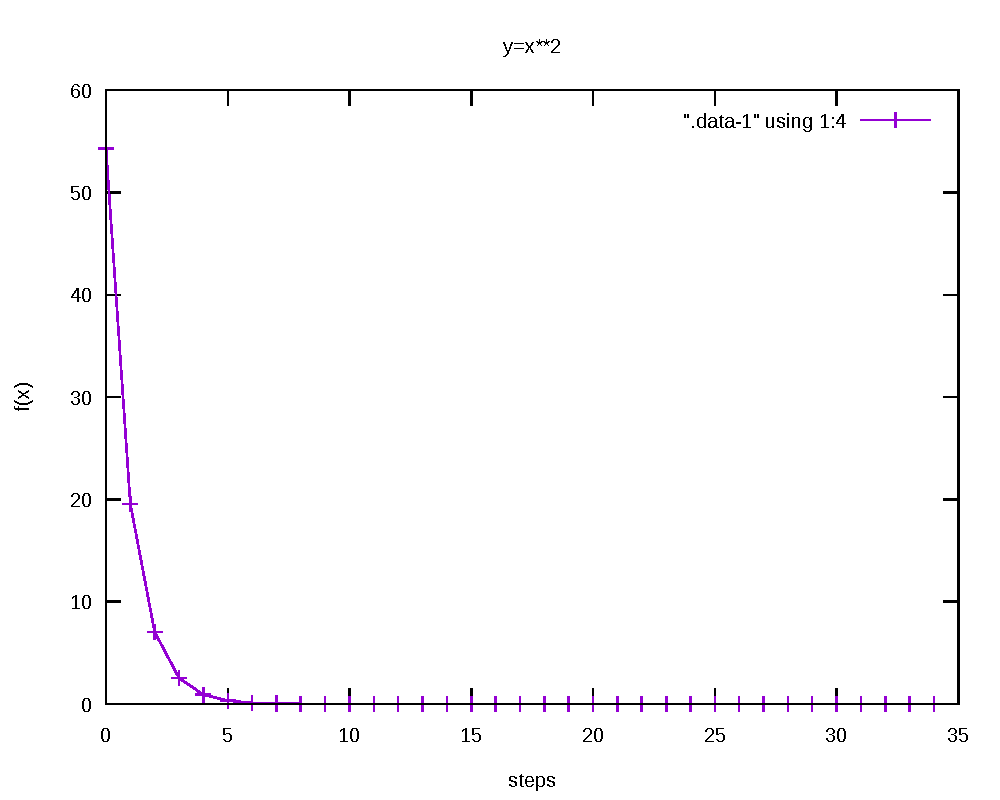
\includegraphics[width=5.0cm]{figs/alpha02.pdf}
    \caption{alpha=0.2での目的関数の推移}
    \label{fig:alpha0.2}
    \end{center}
    \end{minipage}
    
    \begin{minipage}{0.33\hsize}
    \begin{center}
    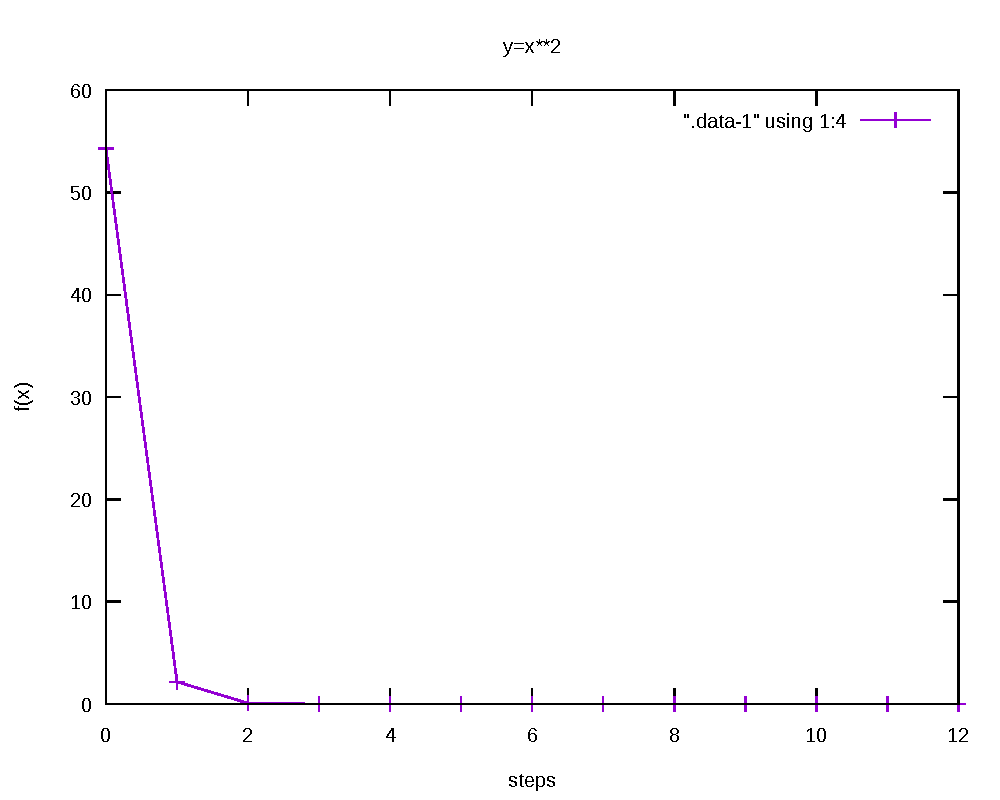
\includegraphics[width=5.0cm]{figs/alpha04.pdf}
    \caption{alpha=0.4での目的関数の推移}
    \label{fig:alpha0.4}
    \end{center}
    \end{minipage}
    
    \begin{minipage}{0.33\hsize}
    \begin{center}
    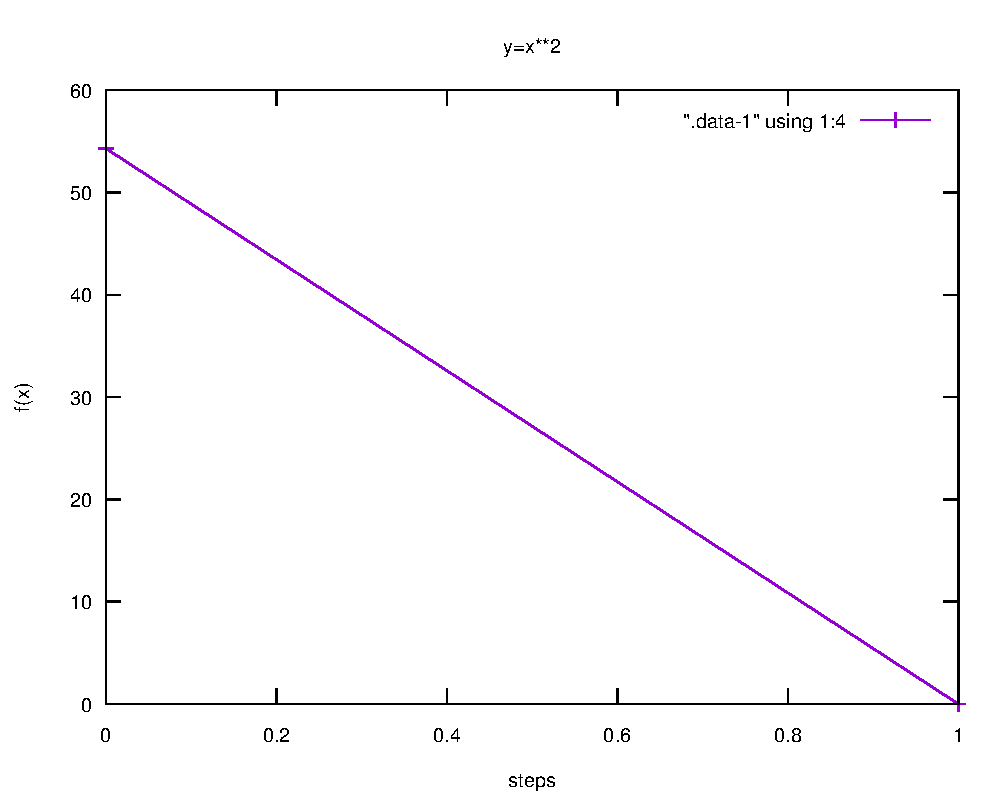
\includegraphics[width=5.0cm]{figs/alpha05.pdf}
    \caption{alpha=0.5での目的関数の推移}
    \label{fig:alpha0.5}
    \end{center}
    \end{minipage}
  \end{tabular}
 \end{center}
\end{figure}

\begin{figure}[h]
 \begin{center}
  \begin{tabular}{c}
    \begin{minipage}{0.33\hsize}
    \begin{center}
    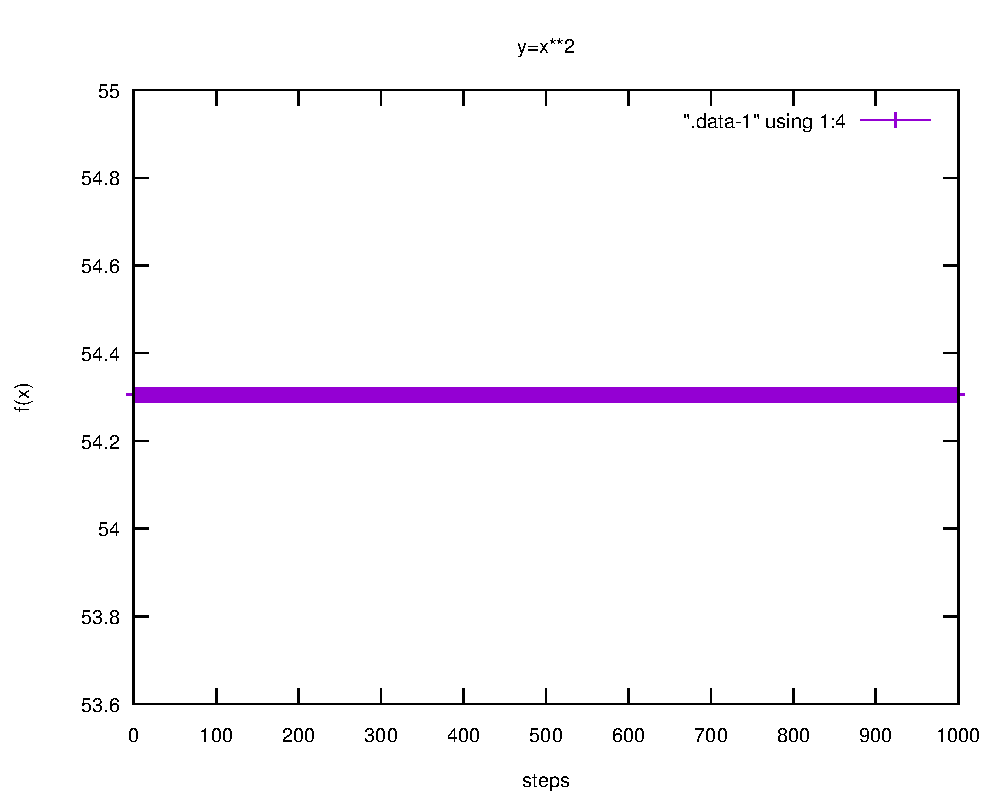
\includegraphics[width=5.0cm]{figs/alpha1.pdf}
    \caption{alpha=1.0での目的関数の推移}
    \label{fig:alpha1.0}
    \end{center}
    \end{minipage}
    
    \begin{minipage}{0.33\hsize}
    \begin{center}
    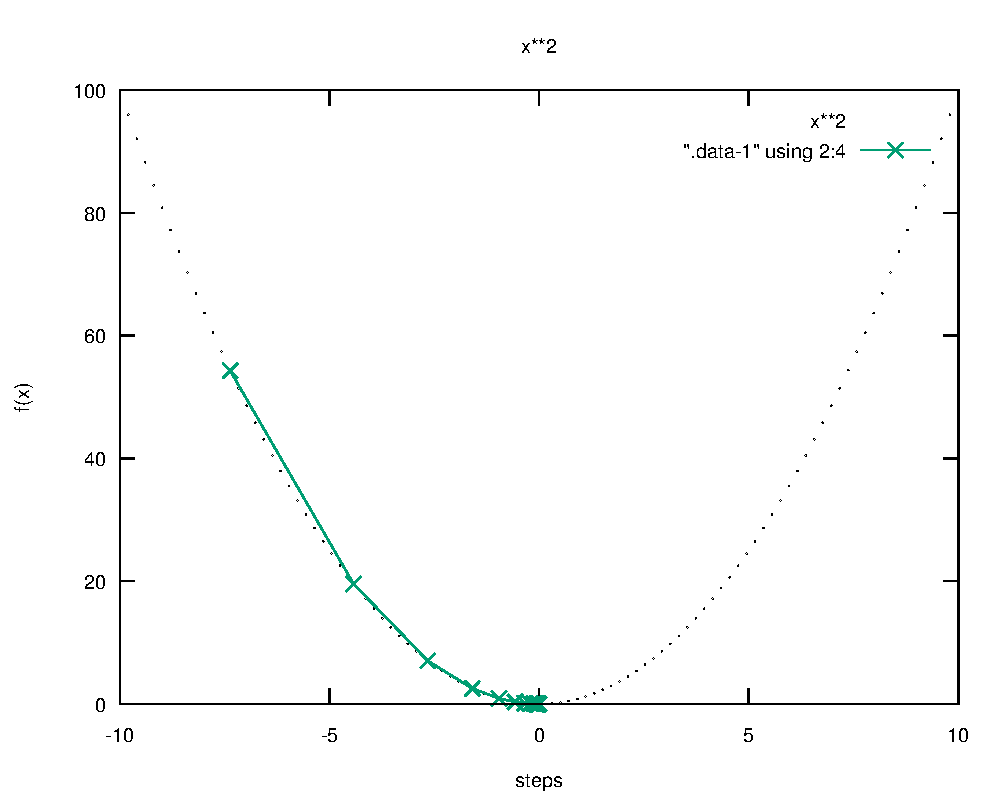
\includegraphics[width=5.0cm]{figs/move_alpha02.pdf}
    \caption{alpha=0.2での探索点の推移}
    \label{fig:move_alpha0.2}
    \end{center}
    \end{minipage}
    
    \begin{minipage}{0.33\hsize}
    \begin{center}
    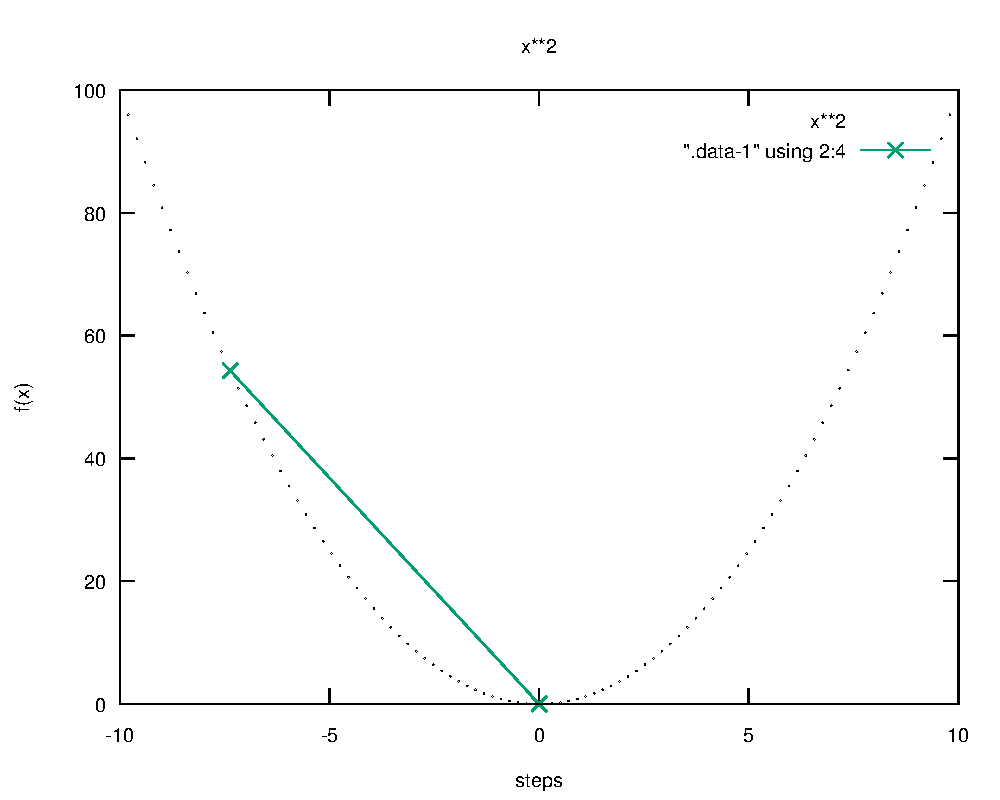
\includegraphics[width=5.0cm]{figs/move_alpha05.pdf}
    \caption{alpha=0.5での探索点の推移}
    \label{fig:move_alpha0.5}
    \end{center}
    \end{minipage}
  \end{tabular}
 \end{center}
\end{figure}